\documentclass[14pt]{beamer}

% TikZ and TikZ libraries to draw Markov chains
\usepackage{tikz}
\usetikzlibrary{automata, positioning}
\usetikzlibrary{arrows.meta}
\usepackage{amssymb}
\usepackage{pifont}
\newcommand{\cmark}{\ding{51}}%
\newcommand{\xmark}{\ding{55}}%
\usepackage[ruled]{algorithm2e}

% Presento style file
\usepackage{config/presento}

% custom command and packages
% custom packages
\usepackage[absolute, overlay]{textpos}
\setlength{\TPHorizModule}{\textwidth}
\setlength{\TPVertModule}{\textwidth}

\newcommand\crule[1][black]{\textcolor{#1}{\rule{2cm}{2cm}}}



% Information
\title{\Large{Optimization vs Epidemics}}
\author{Paul Beaujean\\ \small{joint work with Cristina Bazgan \& \'Eric Gourdin}}
\institute{\small{LAMSADE - Universit\'e Paris-Dauphine \& Orange Labs}}
\date{\textbf{COCOA 2018}  \\ December 16, 2018}

\begin{document}

% Title page
\begin{frame}[plain, noframenumbering]
\maketitle
\hfill
\includegraphics[height=2.5em]{images/lamsade-logo}
\includegraphics[height=2.5em]{images/orange-logo}
\end{frame}

% some context: more malware epidemic than ever, high cost for businesses and governments

\framepic[1]{images/wannacry}{
\begin{textblock}{1}(0.05,0.02)
WannaCry (May 2017)
\end{textblock}
}

\framepic[1]{images/petya}{
\begin{textblock}{1}(0.05,0.07)
Petya (from early 2016 to June 2017)
\end{textblock}
}

\framepic[1]{images/opendaylight}{
\begin{textblock}{1}(0.05,0.05)
SDN: software-defined networking
\end{textblock}
}

\framepic[1]{images/poseidon}{
\begin{textblock}{1}(0.05,0.05)
Poseidon: machine learning for node health
\end{textblock}
}

% mathematical analysis of epidemics in networks

\begin{frame}{SDN against malware}
\begin{fullpageitemize}
\item $\bullet$ transparent and unified data analysis
\item $\bullet$ network management by algorithms
\item $\triangleright$ opportunity to design autonomous security systems for networks
\item $\bullet$ our focus: stopping malware epidemics
\end{fullpageitemize}
\end{frame}

\begin{frame}{Networked epidemic models}
\begin{fullpageitemize}
\item $\bullet$ undirected graph $G = (V,E)$ represents neighborhood of $n := |V|$ nodes
\item $\bullet$ a node is either \textbf{{\color{green}S}}usceptible or \textbf{{\color{red}I}}nfected
\item \begin{center}
\resizebox{5em}{!}{%
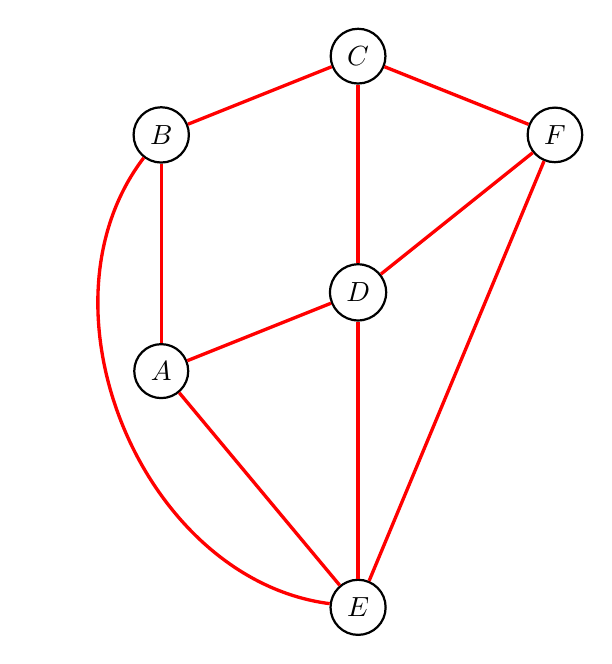
\begin{tikzpicture}
\begin{scope}[every node/.style={circle,thick,draw}]
    \node (A) at (0,0) {$A$};
    \node (B) at (0,3) {$B$};
    \node (C) at (2.5,4) {$C$};
    \node (D) at (2.5,1) {$D$};
    \node (E) at (2.5,-3) {$E$};
    \node (F) at (5,3) {$F$};
\end{scope}

\begin{scope}[>={Stealth[black]},
              every edge/.style={draw=red,very thick}]
    \path [-] (A) edge (B);
    \path [-] (B) edge (C);
    \path [-] (A) edge (D);
    \path [-] (D) edge (C);
    \path [-] (A) edge (E);
    \path [-] (D) edge (E);
    \path [-] (D) edge (F);
    \path [-] (C) edge (F);
    \path [-] (E) edge (F); 
    \path [-] (B) edge[bend right=60] (E); 
\end{scope}
\end{tikzpicture}} \hspace{1em}
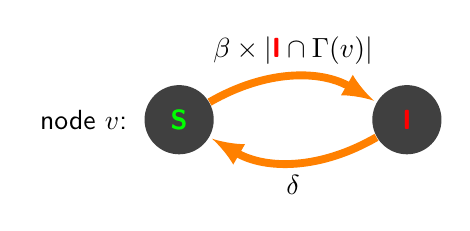
\begin{tikzpicture}[font=\sffamily]
    \node[state,
          text=green,
          draw=none,
          fill=gray!50!black] (S) {\textbf{S}};
	\node[state,
    	  left=0.05cm of S,
    	  text=black,
          draw=none] (v) {node $v$:};
    \node[state,
          right=2cm of S,
          text=red, 
          draw=none, 
          fill=gray!50!black] (I) {\textbf{I}};
 	\draw[every loop,
          auto=left,
          line width=1mm,
          >=latex,
          draw=orange,
          fill=orange]
        (S) edge[bend left]  node {$\beta \times |{\color{red} \textbf{I}} \cap \Gamma(v)|$} (I)
        (I) edge[bend left] node {$\delta$} (S);
\end{tikzpicture}
\end{center}
\item $\bullet$ Markov chain with $2^{n}$ states
\item $\bullet$ unique absorbing state: every node is \textbf{{\color{green}S}}
\end{fullpageitemize}
\end{frame}

\framecard[colorgreen]{{\color{white}
\underline{sufficient} condition for \\ $O(\log n)$ time to extinction:
\vfill
\hugetext{$\lambda_1(G) < \dfrac{\delta}{\beta}$}
\vfill
\hfill
\setnote{
\footnotesize{\textbf{{\color{white} [Prakash et al. '12]}}}
}
}}

\begin{frame}{From a theorem to a control system}
How to achieve $\lambda_1(G) < \dfrac{\delta}{\beta}$?

\begin{fullpageitemize}
\item {\small note: $\beta$ and $\delta$ can be inferred in real time with e.g. maximum likelihood estimators [Ruhi et al. '17]}
\item
\item \textbf{A)} deploy software patches to increase $\delta / \beta$
\item $\to$ {\small hand-crafted response against specific malware}
\item $\to$ {\small hard to predict the effect of a patch on $\beta$ and/or $\delta$}
\item
\item \textbf{B)} modify topology to decrease $\lambda_1(G)$
\item $\to$ {\small generic response against any epidemic}
\end{fullpageitemize}
\end{frame}

\begin{frame}[noframenumbering]{From a theorem to a control system}
How to achieve $\lambda_1(G) < \dfrac{\delta}{\beta}$?
\begin{fullpageitemize}
\item {\small note: $\beta$ and $\delta$ can be inferred in real time with e.g. maximum likelihood estimators [Ruhi et al. '17]}
\item
\item \textbf{{\color{red} A)}} deploy software 
patches to increase $\delta / \beta$
\item $\to$ {\small hand-crafted response against specific malware}
\item $\to$ {\small hard to predict the effect of a patch on $\beta$ and/or $\delta$}
\item
\item \textbf{{\color{green} B)}} modify topology to decrease $\lambda_1(G)$
\item $\to$ {\small generic response against any epidemic}
\end{fullpageitemize}
\end{frame}

\begin{frame}{What is $\lambda_1(G)$?}
\begin{fullpageitemize}
\item \resizebox{8em}{!}{%
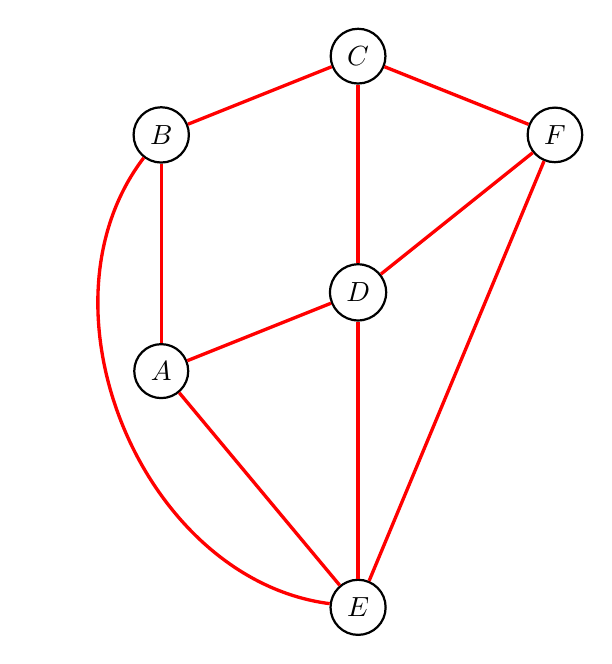
\begin{tikzpicture}
\begin{scope}[every node/.style={circle,thick,draw}]
    \node (A) at (0,0) {$A$};
    \node (B) at (0,3) {$B$};
    \node (C) at (2.5,4) {$C$};
    \node (D) at (2.5,1) {$D$};
    \node (E) at (2.5,-3) {$E$};
    \node (F) at (5,3) {$F$} ;
\end{scope}
\begin{scope}[>={Stealth[black]},
              every edge/.style={draw=red,very thick}]
    \path [-] (A) edge (B);
    \path [-] (B) edge (C);
    \path [-] (A) edge (D);
    \path [-] (D) edge (C);
    \path [-] (A) edge (E);
    \path [-] (D) edge (E);
    \path [-] (D) edge (F);
    \path [-] (C) edge (F);
    \path [-] (E) edge (F); 
    \path [-] (B) edge[bend right=60] (E); 
\end{scope}
\end{tikzpicture}}
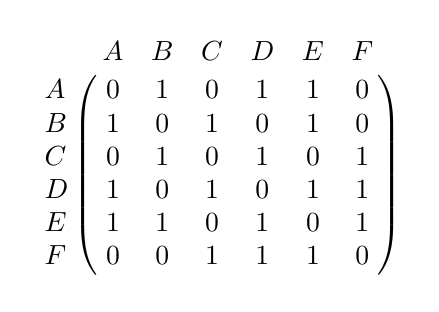
\begin{tikzpicture}
\node (matrix) at (0,0) {
$
\bordermatrix{
  & A & B & C & D & E & F \cr
A & 0 & 1 & 0 & 1 & 1 & 0 \cr
B & 1 & 0 & 1 & 0 & 1 & 0 \cr
C & 0 & 1 & 0 & 1 & 0 & 1 \cr
D & 1 & 0 & 1 & 0 & 1 & 1 \cr
E & 1 & 1 & 0 & 1 & 0 & 1 \cr
F & 0 & 0 & 1 & 1 & 1 & 0 \cr
}$};
\end{tikzpicture}
\item spectrum of the above adjacency matrix:
\item \quad \{ \textcolor{red}{3.39}, 0.19, 0.81, -0.55, -1.57, -2.27 \}
\end{fullpageitemize}
\end{frame}

\begin{frame}{The spectral radius of $G = (V, E)$}
\begin{fullpageitemize}
\item $\bullet$ structural param. related to connectivity
\item \quad $\max\left(\sqrt{\Delta(G)}, \dfrac{2 m}{n} \right) \leq \lambda_1(G) \leq \Delta(G)$
\item
\item $\bullet$ a graph with no edges has $\lambda_1(\mathbf{0}) = 0$
\item
\item \begin{color}{blue} Theorem: $\lambda_1$ is monotone \end{color}
\item \quad if $H$ is a subgraph of $G$ then $\lambda_1(H) \leq \lambda_1(G)$
\item
\item \begin{color}{blue}  Theorem: $\lambda_1$ is positive homogeneous \end{color}
\item \quad if $\alpha > 0$ then $\lambda_1(\alpha \, A) = \alpha \, \lambda_1(A)$
\end{fullpageitemize}
\end{frame}

\begin{frame}{A natural optimization problem}
\begin{fullpagedescription}
\item[Problem:] \textsc{Maximum $\lambda$-spectral Subgraph}
\item[Instance:] undirected graph $G = (V, E)$ and spectral threshold $1 \leq \lambda < \lambda_1(G)$
\item[Task:] find a subgraph $H = (V, E')$ of $G$ with maximum number of edges and $\lambda_1(H) \leq \lambda$
\end{fullpagedescription}
\begin{fullpageitemize}
\item $\bullet$ Set $\lambda = \dfrac{\delta}{\beta}$ to end a given epidemic
\item $\bullet$ NP-hard even in graphs with $\Delta \leq 3$
\end{fullpageitemize}
\end{frame}

\begin{frame}{I always have trouble with}
\begin{center}
    \includegraphics[height=0.87\textheight]{images/design-approx-cover.png}
\end{center}
\end{frame}

\begin{frame}{M$\lambda$SSP as a mathematical program}
\begin{fullpageitemize}
\item \begin{align*}
\max \, & \, \sum_{ij \in E} \, y_{ij} \\
\text{s.t.} \, & \, \sum_{ij \in E} \, y_{ij} \, A_{ij} \preceq \lambda \, I \quad\quad (\mathcal{P}) \\
& \, y_{ij} \in \{0,1\},\, \forall ij \in E
\end{align*}
\end{fullpageitemize}
\begin{fullpageitemize}
\item $\bullet$ recall that $M \succeq N \iff \forall i,\, \lambda_i(M - N) \geq 0$
\item $\bullet$ hence $A \preceq \lambda \, I \iff \lambda_1(A) \leq \lambda$
\item $\bullet$ binary SDP amenable to MISDP solvers
\end{fullpageitemize}
\end{frame}

\begin{frame}{A polytime solvable relaxation}
\begin{fullpageitemize}
\item \begin{align*}
\max \, & \, \sum_{ij \in E} \, y_{ij} \\
\text{s.t.} \, & \, \sum_{ij \in E} \, y_{ij} \, A_{ij} \preceq \lambda \, I \quad\quad\quad (\mathcal{S}) \\
& \, \sum_{j \in \Gamma(i)} y_{ij} \leq \lambda^2,\, \forall i \in V \\
& \, y_{ij} \in [0,1],\, \forall ij \in E
\end{align*}
\end{fullpageitemize}
\begin{fullpageitemize}
\item $\bullet$ valid inequality because: $\lambda_1 \leq \lambda \Rightarrow \Delta \leq \lambda^2$
\item $\bullet$ solvable by fast SDP solvers e.g. SuperSCS
\end{fullpageitemize}
\end{frame}

\begin{frame}{Relaxation \& randomized rounding}
\begin{fullpageitemize}
\item $\bullet$ solve relaxation and let $y^* = \arg \mathcal{S}$
\item $\bullet$ define r.v. $\mathbf{x}_{ij} \sim \text{Bernoulli}(y_{ij}^*/r)$
\item $\bullet$ let $H = \{ij \in E \,|\, x_{ij} = 1\}$
\item $\bullet$ determine $r > 1$ s.t. $H$ is feasible w.h.p. $\Pr(\lambda_1(\sum \mathbf{x}_{ij} A_{ij}) \leq \lambda) = 1 - 1/n$
\item $\triangleright$ randomized $r$-approximation algorithm
\item $\bullet$ oldie but goodie {\small[Raghavan \& Tompson '87]}
\end{fullpageitemize}
\end{frame}

\begin{frame}{Approximate maximization}
\begin{figure}[h]
\centering
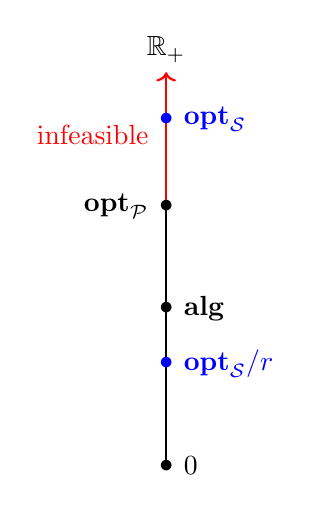
\begin{tikzpicture}
\draw[-,thick,color=red] (0,-2) -- (0,-1.5);
\draw[-,thick] (0,-2) -- (0,1.3);
\draw[->,thick,color=red] (0,1.3) -- (0,3);
\draw (0,3) node[above] {$\mathbb{R}_+$};

\draw[color=blue] (0,2.4) node {$\bullet$};
\draw[color=blue] (0.1,2.4) node[right] {$\textbf{opt}_{\mathcal{S}}$};
\draw[color=red] (-0.1,2.2) node[left] {infeasible};

\draw (0,1.3) node {$\bullet$};
\draw (-0.1,1.3) node[left] {$\textbf{opt}_{\mathcal{P}}$};

\draw (0,0) node {$\bullet$};
\draw (0.1,0) node[right] {$\textbf{alg}$};

\draw[color=blue] (0,-0.7) node {$\bullet$};
\draw[color=blue] (0.1,-0.7) node[right] {$\textbf{opt}_{\mathcal{S}} / r$};

\draw (0,-2) node {$\bullet$};
\draw (0.1,-2) node[right] {0};
\end{tikzpicture}
\caption{\textbf{alg} is the expected number of edges in $H$}
\label{relaxation-rounding}
\end{figure}
\end{frame}

\begin{frame}{Determining the approx. ratio $r$}
\begin{fullpageitemize}
\item $\bullet$ instead of designing algorithms\ldots
\item $\triangleright$ prove concentration for a random object!
\item $\bullet$ here: random adjacency matrices
\item $\bullet$ use concentration inequalities for sum of random matrices $\mathbf{X} = \sum_e \mathbf{X}_{e}$ {\small[Tropp '15]}
\item \begin{equation*}
\Pr( \lambda_1(\mathbf{X}) \geq a) \leq \min_{t > 0} e^{-t a} \text{tr} \exp \left( \sum_e \log\left(\mathbb{E} e^{t \mathbf{X}_e}\right) \right)
\end{equation*}
\end{fullpageitemize}
\end{frame}

\begin{frame}{Matrix Bernstein gives}
\begin{fullpageitemize}
\item $\bullet$ for $\mathbf{X} = \sum_e \mathbf{X}_{e}$ with $\mathbb{E} \mathbf{X} = \mathbf{0}$ and $\lambda_1(\mathbf{X}_e) \leq L$
\item $\bullet$ matrix variance: $v(\mathbf{X}) \stackrel{\text{def}}{=}  \lambda_1(\sum_e \mathbb{E} \mathbf{X}_e^2)$
\begin{equation*}
    \Pr(\lambda_1(\mathbf{X}) \geq a) \leq
n \exp\left(-\dfrac{a^2}{2v(\mathbf{X}) + 2L a/3}\right)
\end{equation*}
\item $\bullet$ apply to $\bar{\mathbf{A}} = \sum \mathbf{x}_{ij} A_{ij} - \mathbb{E}\mathbf{x}_{ij} A_{ij}$, $a = (1 - 1/r) \lambda$
\item \textbf{Goal:} $\Pr(H \text{ is infeasible}) \leq 1/3$
\end{fullpageitemize}
\end{frame}

\begin{frame}[noframenumbering]{Matrix Bernstein gives}
\begin{fullpageitemize}
\item $\bullet$ for $\mathbf{X} = \sum_e \mathbf{X}_{e}$ with $\mathbb{E} \mathbf{X} = \mathbf{0}$ and $\lambda_1(\mathbf{X}_e) \leq L$
\item $\bullet$ matrix variance: $v(\mathbf{X}) \stackrel{\text{def}}{=}  \lambda_1(\sum_e \mathbb{E} \mathbf{X}_e^2)$
\begin{equation*}
    \Pr(\lambda_1(\mathbf{X}) \geq a) \leq
n \exp\left(-\dfrac{a^2}{2v(\mathbf{X}) + 2L a/3}\right)
\end{equation*}
\item $\bullet$ apply to $\bar{\mathbf{A}} = \sum \mathbf{x}_{ij} A_{ij} - \frac{y_{ij}^*}{\mathbf{{\color{red} r}}} A_{ij}$, $a = (1 - 1/\mathbf{{\color{red} r}}) \lambda$
\item \textbf{Goal:} $\Pr(H \text{ is infeasible}) \leq 1/3$ for $\mathbf{{\color{red} r}} = \,?$
\end{fullpageitemize}
\end{frame}

\begin{frame}{$r = O(\log n)$ when $\lambda \geq \log n$}
\begin{fullpageitemize}
\item $\bullet$ key property: $v(\bar{\mathbf{A}}) \leq \lambda^2 / r$ (cf. valid ineq.)
\item $\bullet$ crank out the math\ldots
\item \textbf{Result:} $\Pr(H \text{ is infeasible}) \leq 1/3$ for $r = 1 + 3\log n$ if $\lambda \geq \log n$
\item $\bullet$ from $1/3$ to $1/n$ with amplification
\end{fullpageitemize}
\end{frame}

\begin{frame}{What about $\lambda \leq \log n$?}
    \begin{fullpageitemize}
    \item $\bullet$ spectral ver. of classical result on $\Delta$ vs $\nu$ \begin{equation*}
    \nu(G) \geq \frac{m}{\lambda_1^2(G) - 1}
    \end{equation*}
    \item $\bullet$ implies that a maximum matching is a $(\lambda^2 - 1)$-approximation of M$\lambda$SSP
    \item \textbf{Result:} $O(\log^2 n)$-approx. if $\lambda \leq \log n$
    \end{fullpageitemize}
\end{frame}

\begin{frame}{Conclusion}
\begin{fullpageitemize}
\item $\bullet$ randomized $O(\log^2 n)$-approximation algorithm
\item $\bullet$ parallel approximate SDP solver + parallel independent rounding + power method
\item $\bullet$ super fast in practice, can exploit GPUs
\item 
\end{fullpageitemize}
\end{frame}

\begin{frame}{Perspectives}
\begin{fullpageitemize}
\item $\bullet$ hardness of approx. (Max $k$-Cut?)
\item $\bullet$ Erd\"os-R\'enyi graphs limit our approach:
\begin{equation*}
    \lambda_1(G(n,p)) = \Theta\left(\sqrt{\dfrac{\log n}{\log \log n}} \right)
\end{equation*}
even when $np = O(1)$ {\small[Krivelevich et al. '01]}
\item $\bullet$ maximum degree-constrained subgraph for $\lambda \leq \log n$ (from $\lambda^2$ to $\lambda$-approx?)
\item $\bullet$ better concentration bounds? {\small[Le et al., '15]}
\end{fullpageitemize}
\end{frame}

\framepic[0.8]{images/epidemic}{
 \begin{textblock}{8}(0.3,0.5)
    {\color{white}\hugetext{Any questions?}}
 \end{textblock}
}

% \begin{frame}{i.i.d. Bernoulli on a regular graph}
% \begin{center}
% \includegraphics[height=0.87\textheight]{images/sampling-rr}
% \end{center}
% \end{frame}

% \begin{frame}{i.i.d. Bernoulli on an irregular graph}
% \begin{center}
% \includegraphics[height=0.87\textheight]{images/sampling-ba}
% \end{center}
% \end{frame}

% \begin{frame}{Power of SDP relaxation}
% \begin{center}
% \includegraphics[height=0.87\textheight]{images/karate-sdp-vs-bernoulli}
% \end{center}
% \end{frame}

\begin{frame}[plain, noframenumbering]{Problem variants}
\begin{fullpageitemize}
\item $\bullet$ spectral subgraph setting with two parameters: number of edges vs spectral radius
\item \begin{table}
\begin{tabular}{ l|c|c } 
& constraint & objective \\ 
\hline
v. Mieghem et al. '12 & $|E'| = k$ & $\min \lambda_1$ \\ 
Saha et al. '15 & $\lambda_1 \leq \lambda$ & $\min |E| - |E'|$ \\
Zhang et al. '15 & $|E'| \leq k$ & $\min \lambda_1$ \\ 
this work & $\lambda_1 \leq \lambda$ & $\max |E'|$
\end{tabular}
\end{table}
\end{fullpageitemize}
\end{frame}

\begin{frame}[plain, noframenumbering]{The Laplacian spectrum}
\begin{fullpageitemize}
\item $\bullet$ $\mu \leq \mu_2(H)$ instead of $\lambda_1(H) \leq \lambda$
\item $\bullet$ related to expander construction: \begin{align*}
\min \, & \, \sum_{ij \in \bar{E}} \, y_{ij} \\
\text{s.t.} \, & \, L(G) + \sum_{ij \in \bar{E}} \, y_{ij} \, L_{ij} \succeq \mu \, P_{\mathbf{1}^{\perp}} \quad (\mathcal{Q}) \\
& \, y_{ij} \in \{0,1\},\, \forall ij \in \bar{E}
\end{align*}
\item $\bullet$ some results \small{[Ghosh \& Boyd '06, Kolla et al. '09]}
\end{fullpageitemize}
\end{frame}

\framepic[0.8]{images/sampling1}{}

\end{document}